% titlepage is included by Makefile from parent directory


\pagebreak
\section*{Preface}
 RexIO is library for console (rogue-like) user interfaces for
 applications such as adventure games, full-screen editors, business
 software etc. providing support for vast variety of terminals and
 connection types (unified interface for local and remote terms,
 support for TERMINFO® database and more).  

 It also provides extensive UI development framework including support
 for forms, toolbars, subwindows frames etc, full internationalization
 support including UNICODE™ compliance as well as CJK character
 properties. Library combines reboustness of modern GUI toolkits and
 efficiency of console-based IO providing comprehensive solution for
 virtually any modern software platform.

 This paper is an introductory tutorial covering several use cases of
 this library as well as description of it's basic features, concepts
 and internat structure. Please refer to enclosed source code listing
 and reference manual when anything is unclear.
 
 \vspace{\fill}
\pagebreak
 \subsection*{Symbols}
 \important means, that specific piece of information is important
 \vspace{0.4cm}

 \fullcode indicates a complete program source code, that may be
 compiled and run
 \vspace{0.4cm}

 \advanced indicates an advanced topic, that is not necessary in basic
 usage of library
 \vspace{\fill}
\pagebreak
\tableofcontents 
 \vspace{\fill}\cleardoublepage
\lstset{commentstyle=\textit,stepnumber=1 ,keywordstyle=\bfseries,
    showstringspaces=false}
\lstset{numbers=left,numbersep=0.1cm,numberstyle=\tt,tabsize=4,
    basicstyle=\tt\footnotesize,texcl=false}
\lstset{language=C++,breaklines=true}
\pagestyle{headings}
\section{General layout of library}
\subsection {Possibilities}
  The library consists of two basic functional blocks: The connectivity
  module (librexio) and user interface toolkit (librexiotk). The first
  provides unified interface to screen, while second provides
  extensive set of extensible
  utility classes representing some specific interface
  functionality. Figure below represents typical layout of these items:
  \index{layout}

  \begin{figure}[H]
  \begin{center}
  \leavevmode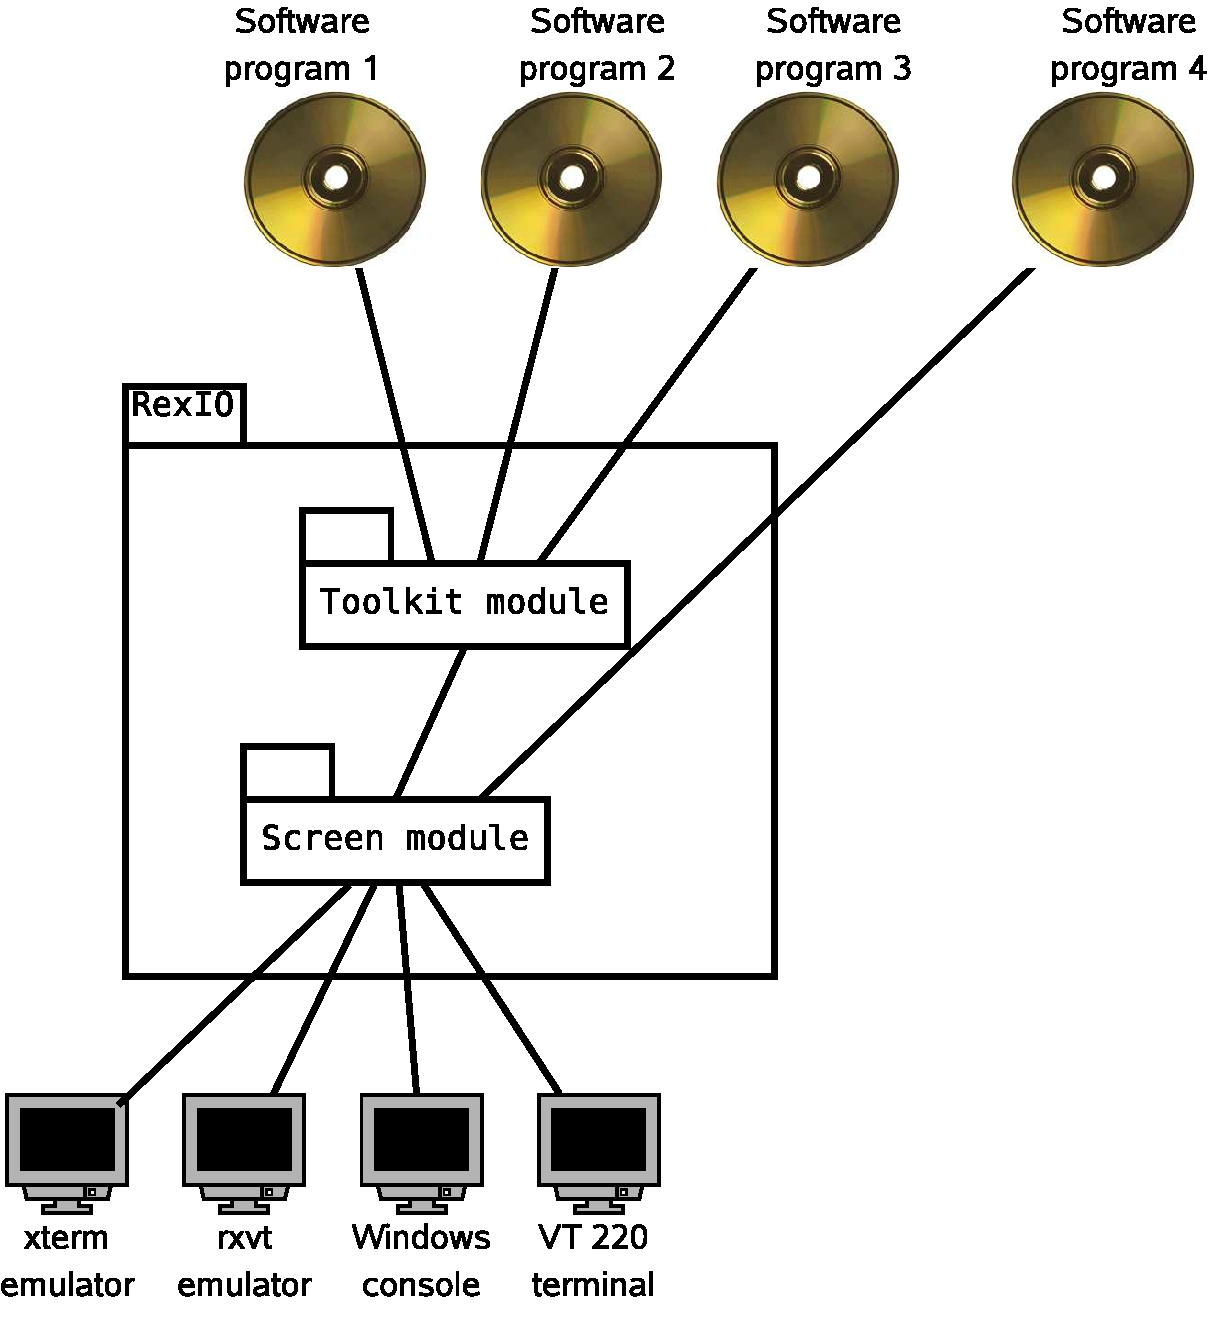
\includegraphics[width=200pt]{graphics/PurposeOfLibrary}
  \end{center}
  \end{figure}

  As you can see, library aims to provide interface to many different
  terminal types, and serve as many software applications as possible.


  Thanks to being object oriented and thread safe, library may allow
  single instance of software program communicate with many clients
  and provide them user interface:

  \begin{figure}[H]
  \begin{center}
  \leavevmode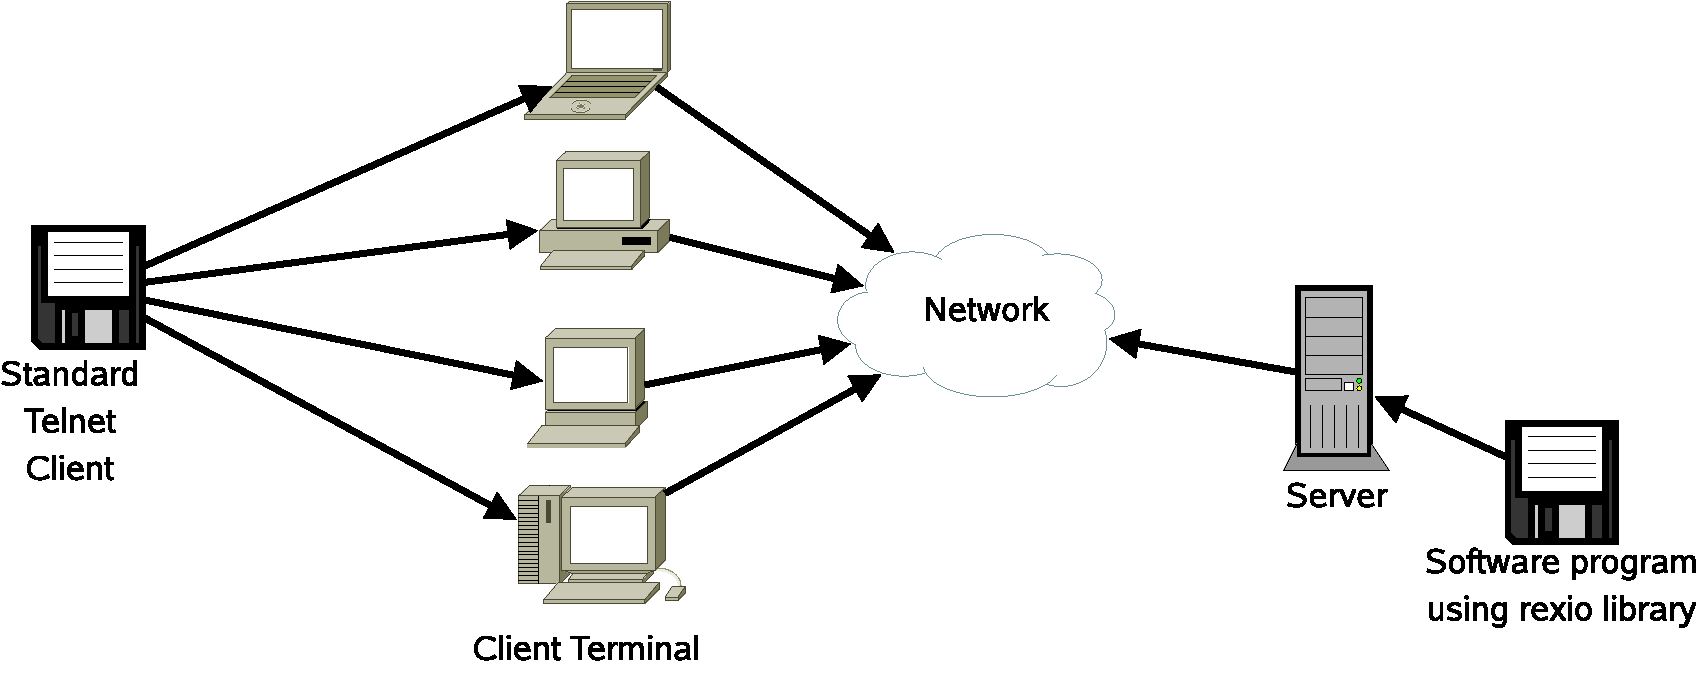
\includegraphics[width=350pt]{graphics/IdeaOfMUD}
  \end{center}
  \end{figure}
  \index{MUD}

  This gives an amazing possibility to create multi user business
  software, collaborative text editors, and also  MMO roleplaying games
  combining availability of traditional MUD's with easy user interface
  of rogue like games. 

\subsection{Internal layout}
  Layout of functional blocks in screen module is as follows:
  \index{subsystems}
  
  \begin{figure}[H]
  \begin{center}
  \leavevmode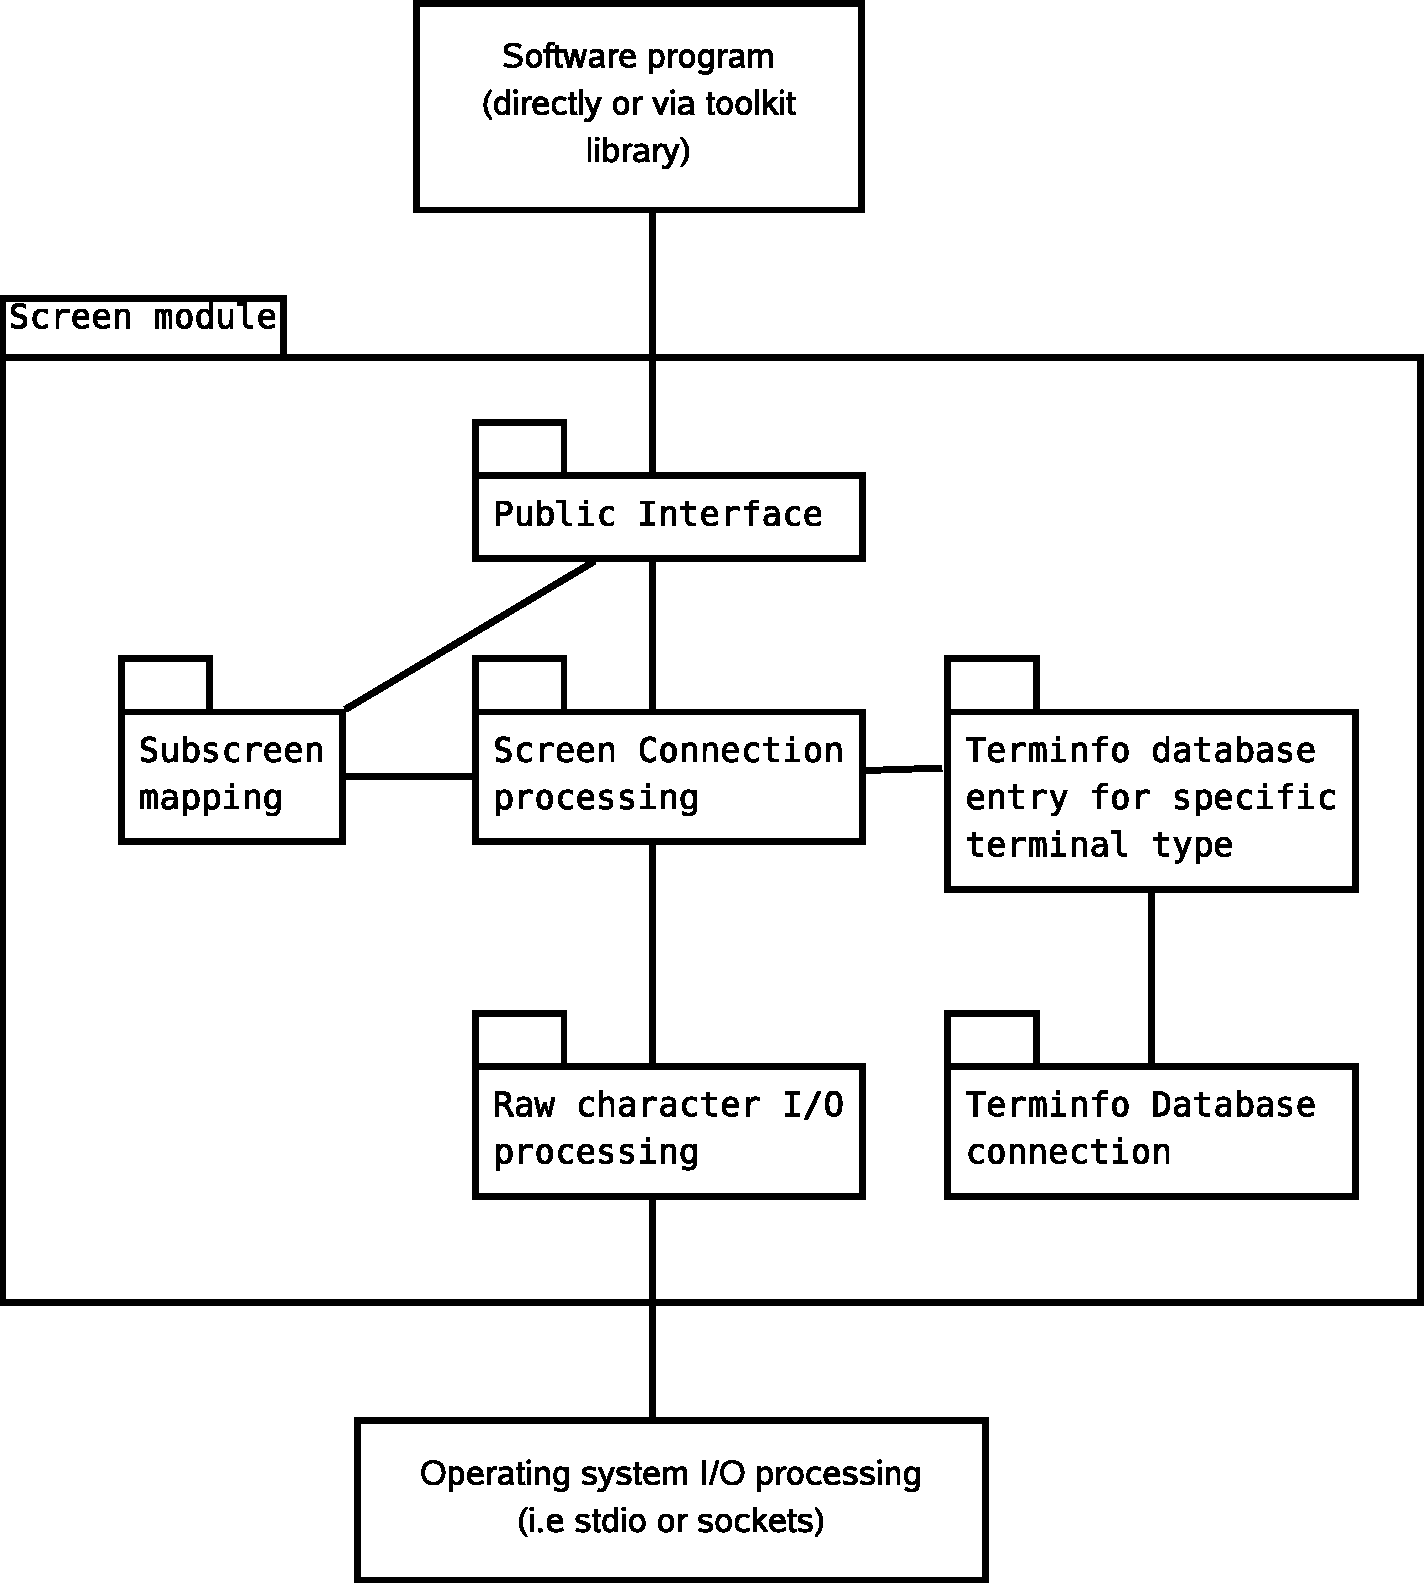
\includegraphics[width=280pt]{graphics/ModuleLayout}
  \end{center}
  \end{figure}
  Each of them is implemented as set of classes with specific
  interfaces between them. Some design principles with brief rationale
  are provided in subsequent sections.


\subsubsection{Thread safety}
  note: ,,module'' symbol in following diagram depicts single instance
  of specific subsystem (functional block):
  \index{thread}
  \advanced

  \begin{figure}[H]
  \begin{center}
  \leavevmode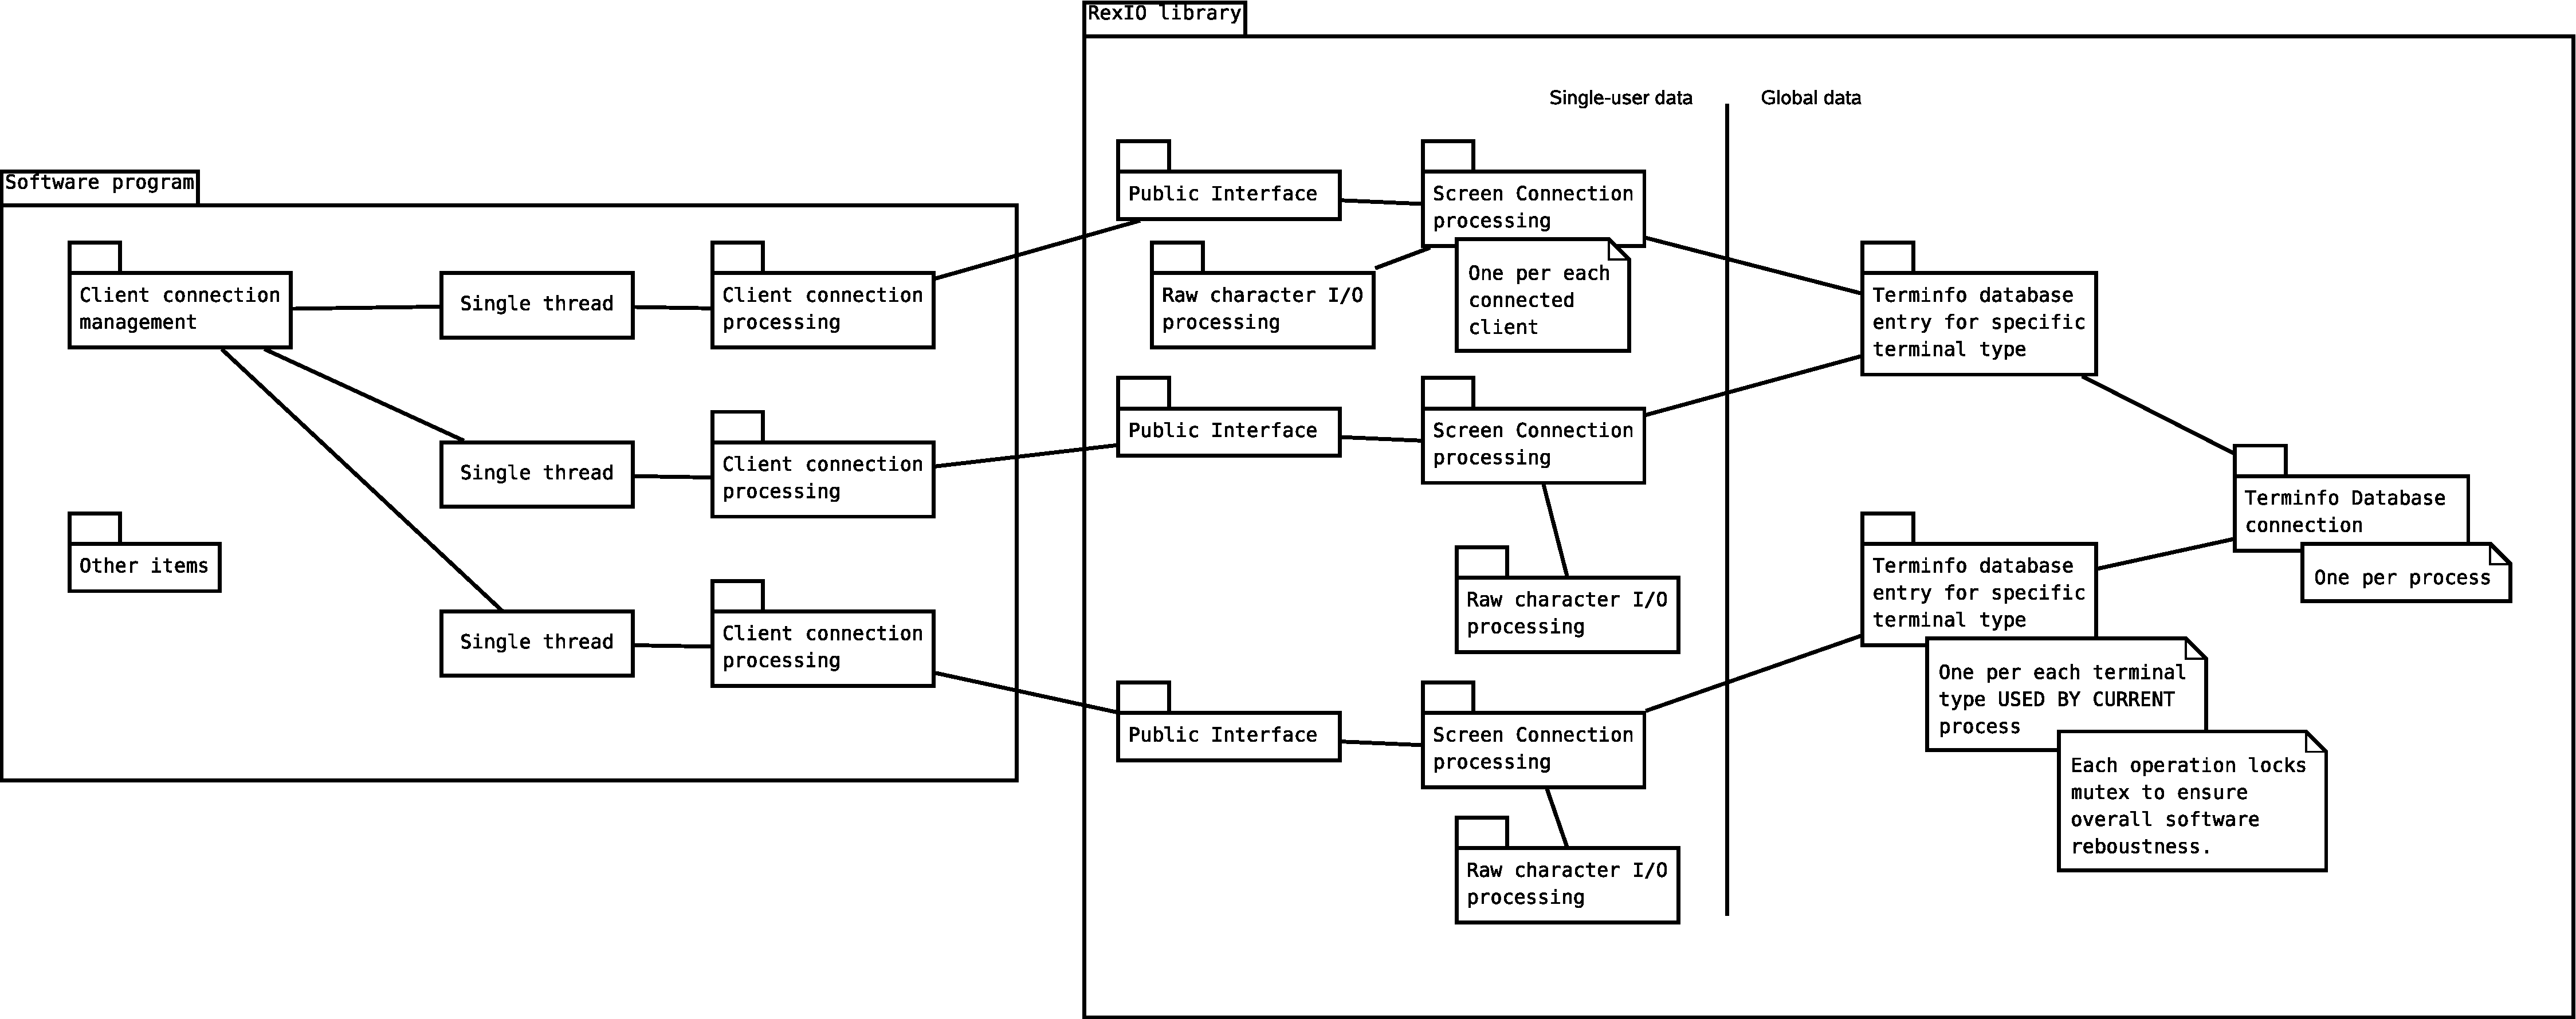
\includegraphics[width=540pt,angle=270]{graphics/MultiThread}
  \end{center}
  \end{figure}
  
  \pagebreak

  Figure on previous page describes typical layout of
  multi-threading-connected features, as well as measures taken to
  obtain stability in threaded programs and ensure their reasonable
  performance.

  As it can be seen, only global data structures are connected to
  TERMINFO database processing, and other items are separated (one per
  connection) to achieve reasonable compromise between versatility and
  efficiency.

  \important
  General guidelines for writing threaded applications using this
  library are as follows:
  
  \begin{itemize}
  \item multiple connections may be created and simultaneously
    processed in multiple threads (guaranteed by library design).
  \item multiple operations at the same moment for SINGLE connection
    are not guaranteed by library design, and therefore special
    measures must be taken while designing software program that uses
    this approach. 
  \end{itemize}
  

\subsubsection{Screen connection processing}
  Screen class generalizes basic screen operations. Support for
  different screen and connection types is implemented through
  inheritance with  multiple polymorphism. RScreen (Real Screen
  Implementation) template generalizes this idea while still allowing
  to take advantage of OOP (Object Oriented Programming).
  \index{subsystems}

  Typical instance of RScreen template looks like this:

  \begin{figure}[H]
  \begin{center}
  \leavevmode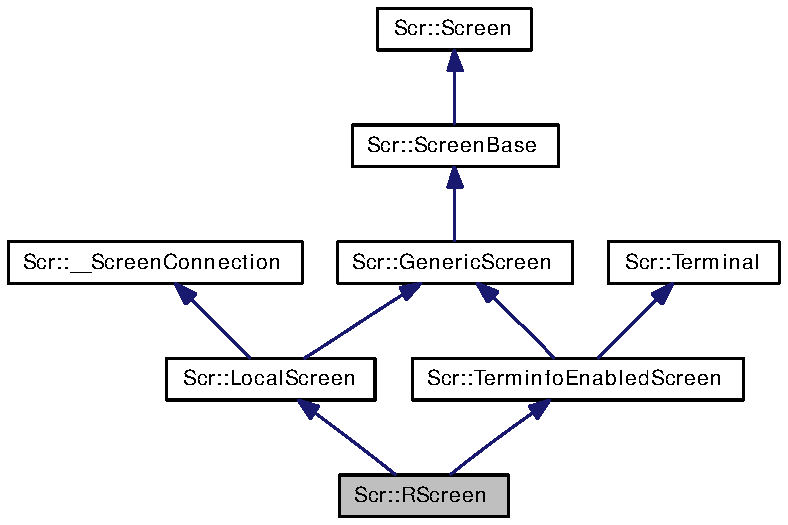
\includegraphics[width=200pt]{graphics/classScr_1_1RScreen__inherit__graph}
  \end{center}
  \end{figure}

  Please note, that fully implementing all this functionality almost
  always involves multitude of object. For example simplified
  collaboration diagram for RScreen implementing local screen that is
  using TERMINFO database looks as follows:

  \begin{figure}[H]
  \begin{center}
  \leavevmode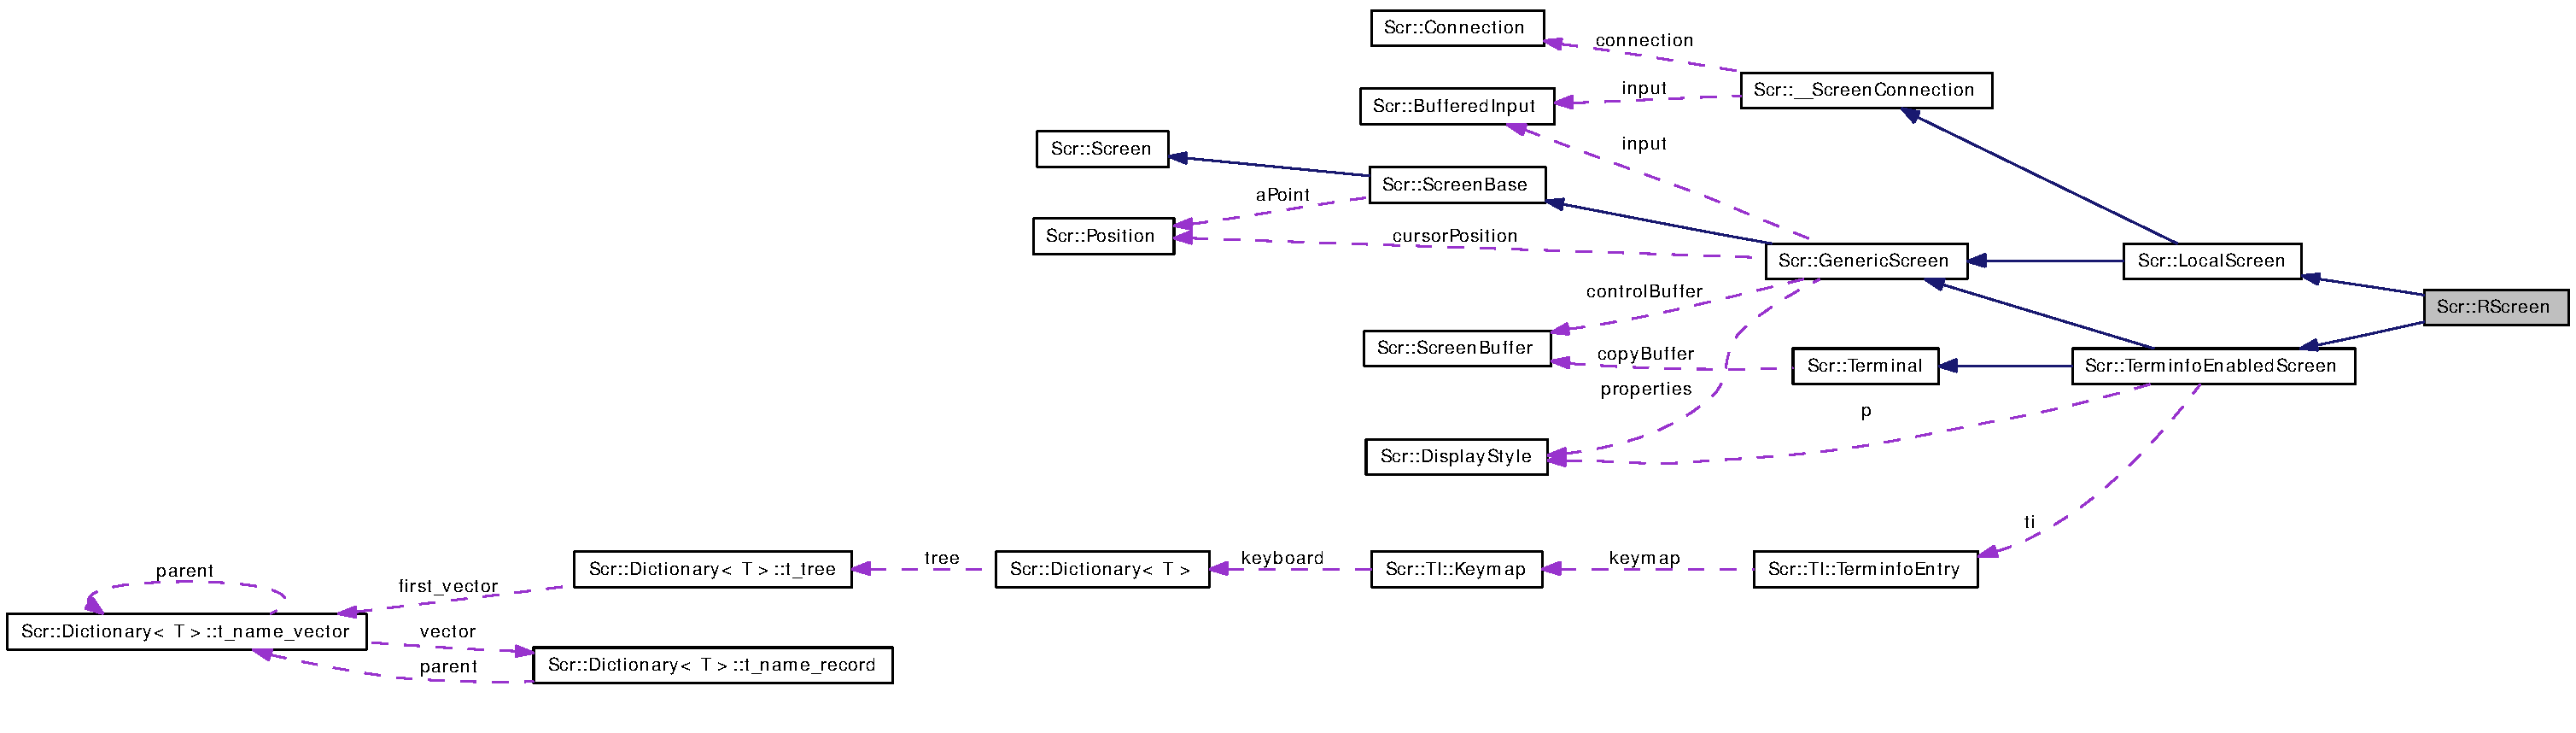
\includegraphics[width=580pt,angle=270,trim=560pt 0 0 0,clip=true]{graphics/classScr_1_1RScreen__coll__graph}
  \end{center}
  \end{figure}

\subsubsection{Sub screen mapping}
  \begin{figure}[H]
  \begin{center}
  \leavevmode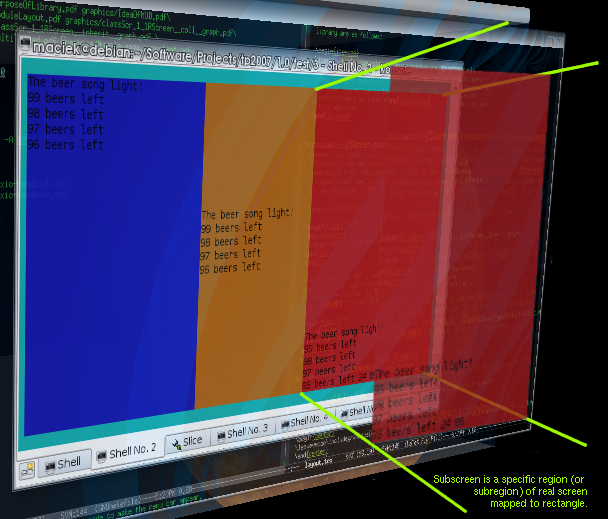
\includegraphics[width=270pt]{graphics/SubscreenMapping}
  \end{center}
  \end{figure}
  \index{subscreen}
  \index{screenshot}
  To fully unite interface and provide efficient way  of designing
  hierarchical display  structures (as user interfaces) concept of
  sub-screen is introduced. Sub-screen is section of screen and is
  itself representative of class screen (inheritance-and-composition
  pattern). 

  \important

  Each basic operation supported by screen is also supported by
  subscreen, as it inherits its interface. Each subscreen operation
  is therefore executed on physical screen with appropriate coordinate
  mapping. Most of these operations affects real screen directly, as
  subscreen doesn't have its own buffer (therefore active point
  coordinates of real screen are not preserved after writing on
  subscreen).

  Please refer to Reference Manual for further details.

\subsubsection{UI Toolkit}
  Scr::Tk namespace contains Widget class that is base to all UI toolkit elements
  Following diagrams demonstrate most of Widget descendents:


  \begin{figure}[H]
  \begin{center}
  \leavevmode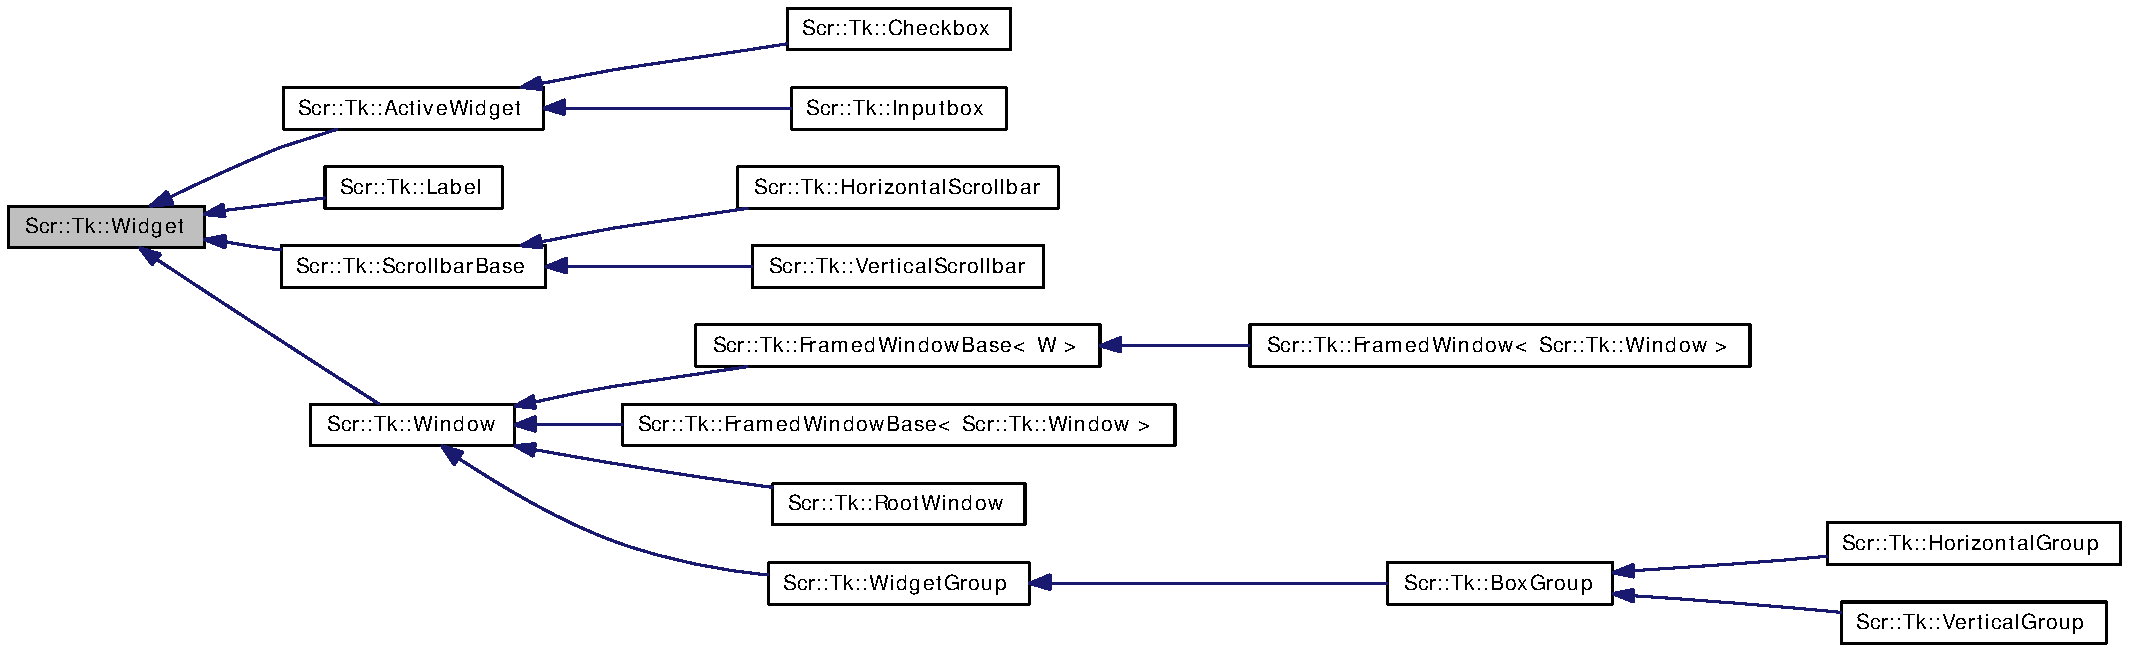
\includegraphics[width=\linewidth,trim=0 0 430pt  0,clip=true]{graphics/classScr_1_1Tk_1_1Widget__inherit__graph}
  \end{center}
  \end{figure}
  \index{toolkit}


  \begin{figure}[H]
  \begin{center}
  \leavevmode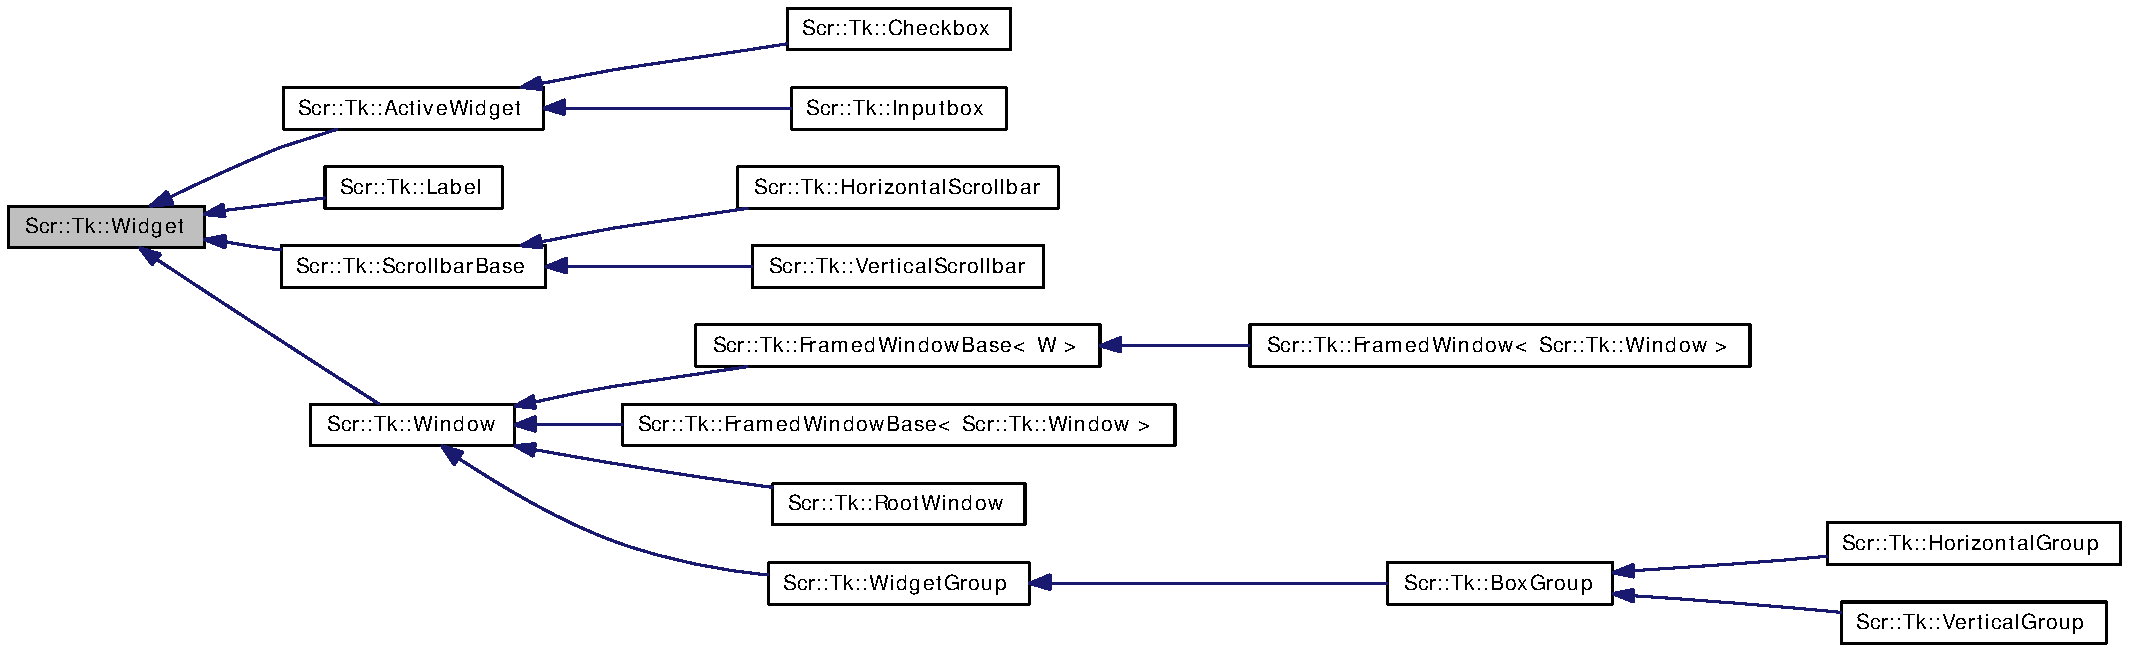
\includegraphics[width=\linewidth,trim=250pt  0  0 150pt ,clip=true]{graphics/classScr_1_1Tk_1_1Widget__inherit__graph}
  \end{center}
  \end{figure}

  Each of them is placed in RootWindow
  
  \begin{figure}[H]
  \begin{center}
  \leavevmode\includegraphics[width=\linewidth]{../latex/classScr_1_1Tk_1_1RootWindow__coll__graph}
  \end{center}
  \end{figure}


% LocalWords:  namespace

\cleardoublepage
\section{Compiling}
To compile this software library you need:

\begin{itemize}
\item POSIX compatible operating system
\item C++ compiler
\item boost libraries (memory and threads)
\item cmake build system
\end{itemize}

When these dependencies are satisfied, you may try to generate UNIX
makefile using following command (dot is important - it represents
,,current path'') in root directory.
\index{cmake}
\index{compile}
\begin{verbatim}
cd **Directory, where RexIO is unpacked**
cmake .
\end{verbatim}

When they are finally  generated, program is compiled in usual way

\begin{verbatim}
make
\end{verbatim}

\index{install}
When 1.0 release candidate will be ready, install target will be added
enabling you to install this library in your system with all other
libraries, and use it for all your programs by just typing

\begin{verbatim}
make install
\end{verbatim}

When for some reason you will decide, you do not need this library
anymore, you may type

\begin{verbatim}
make uninstall
\end{verbatim}


\subsection{Linking your programs against RexIO library}

\begin{verbatim}
g++ yourprogram youroptions -lrexio -lrexiotk
\end{verbatim}
\cleardoublepage

\section{Screen operations basics}
\subsection {Typical program layout - message processing pipeline}
Typical software program consists of many functional components, that
is i.e. some file-reading component, networking subsystem, many other
items... and last, but not least, user interface. In object oriented
languages, such as C++, many of them are implemented as classes, so no
surprise, RexIO is designed to let programmers take advantage of OOP
in user interface design. 

As a result each UI element is implemented as OBJECT, and each
customized element is represented by custom class. Therefore designing
user interface is explicitly designing class implementing specific
interface. Typical UI design is as follows

{\footnotesize\begin{verbatim}
Specific window type ``MyWindow'' is a RootWindow
  When it is resized, 
    it does some action

  When key is pressed, 
    it stores it's code if it is a letter
    program quits if it is Esc

  When it has to display its contents
    it displays stored value
\end{verbatim}}

Design above may be directly converted to C++ code as follows

\begin{lstlisting}
class MyWindow: public RootWindow
{
private:
	int code;
public:
	MyWindow()
		:RootWindow(std::cin,std::cout)
	{
		code=0;
	}


	void OnResize()
	{
		;//do something
	}

	void  OnKeyDown(Key key)
	{
		if (key == Key::Escape)
			Exit(0);
		else if (key.IsABasicKey())
			code=key;
	}

	void OnRedraw(Scr::Screen &screen)
	{
		screen << Clear << GotoYX(2,2) << code << Refresh;
	}

	~MyWindow(){;}
};//MyWindow
\end{lstlisting}

\index{class}
Code above depicts almost complete RexIO application. Full program is as follows:
\fullcode
\begin{lstlisting}
#include<rexio/tk/toolkit.h++>
#include<iostream>
using namespace std;
using namespace Scr;
using namespace Scr::Tk;
using namespace Scr::Control;

class MyWindow: public RootWindow
{
private:
	int code;
public:
	MyWindow()throw()  		// empty specification of
							// throw() means, that function
        					// is not allowed to throw
							// any exceptions.
		:RootWindow(cin,cout)
	{
		code=0;
	}

	void OnResize()throw()
	{
		;//do something
		RootWindow::OnResize();
	}

	void  OnKeyDown(Key key)throw()
	{
		if (key == Key::Escape)
			Exit(0);
		else if (key.IsABasicKey())
			code=key;
		RootWindow::OnKeyDown(key);
	}

	void OnRedraw(Scr::Screen &screen)throw()
	{
		try
		{
			screen << Clear << GotoYX(2,2) << code << Refresh;
		}
		catch (...)
		{
			Exit(1);
		}
	}
	
	~MyWindow()throw(){;}
};//MyWindow

int main (Uint argc,char ** argv)
{
	RootWindow * app = new MyWindow;	
	int result = app->Start(argc, argv);	
	delete app;
	return result;
}
/*end of main function of program*/ 
\end{lstlisting}

As you can see, line 
\vspace{-10pt}\begin{verbatim}
#include<rexio/tk/toolkit.h++>
\end{verbatim}
\vspace{-10pt}includes most general library header file (please note, that this file
includes virtually ,,everything'' - there are also files declaring specific
classes)

\index{namespace}
lines 
\vspace{-10pt}\begin{verbatim}
using namespace std;
using namespace Scr;
using namespace Scr::Tk;
using namespace Scr::Control;
\end{verbatim}
\vspace{-10pt}aren't necessary to make code working, however they allow to simplify
many statements.

Keyword
\vspace{-10pt}\begin{verbatim}
throw
\end{verbatim}
\vspace{-10pt}is used in whole library to specify allowed exception sets, and
therefore enable controlling exception flow. 

Sometimes, when redefining default behavior of windows (especially
RootWindow) it is recommended to call default function after (sometimes
before) custom processing:\vspace{-10pt}
\begin{verbatim}
RootWindow::OnKeyDown(key);
\end{verbatim}

\vspace{\fill}
\pagebreak
\subsection {Basic character output}
\index{output}

\index{stream}
In previous section we have discussed basic printing text
using following sequence
\begin{lstlisting}
screen << Clear << GotoYX(2,2) << "Hello World" << Refresh;//>>
\end{lstlisting}

The same effect may be obtained using plain virtual function calls
\begin{lstlisting}
screen.Clear();
screen.GotoYX(2,2);
screen.AddText("Hello World");
screen.Refresh();
\end{lstlisting}


Please note, that there are multiple (to be precise: 6) variants of
AddText: let us consider two of them
\begin{lstlisting}
virtual void AddText(const char * text)   
virtual void AddText(const wchar_t * text) 
\end{lstlisting}

One of them accept C-style string with one-byte-per-character, and
second accepts wchar\_t (for Linux 4 byte, for Windows 2 byte). 

\index{Jožin z bažin}
The second may be used to print text with diacritics. i.e. to print
,,Jožin z bažin'' you have to type following code:

\noindent{\tt\scriptsize screen.AddText(L"Jožin z bažin");}


\index{UCS}
However as many real software solutions depend on UTF-8 encoding,
specific functionality \textbf{is provided out of the box} 
\begin{lstlisting}
screen.AddText("Jo\xC5\xBEin z ba\xC5\xBEin");
\end{lstlisting}
does exactly, what you may expect
\index{UTF-8}
\index{color}
If you want to emphasize "bažin", you may use following code to add colors:
\begin{lstlisting}
screen << "Jo\xC5\xBEin z " << Fg::Bright << Fg::Red << "ba\xC5\xBEin";//>>
\end{lstlisting}


\index{stream}
SetFgStyle and SetFgColor functions may be called instead of using
this iostream-like syntax. Maybe you won't gain any bigger performance
using these functions, but certainly you may improve control of
overall layout. Also there are functions like Screen::HorizontalLine
simplifying for example box drawing. 

\important
Each of these  functions provides range checking, and throws specific
exception when range is violated. It is recommended to use try-catch
statements to detect such problems and provide rock-solid programs that
virtually never fail. 

%w razie wolnego czasu coś o CJK napisać trzeba

\vspace{\fill}
\pagebreak


\subsection {Component-based hierarchical layout}


\index{component}

To improve your understanding of hierarchical layout (basics of
Scr::Tk::Widget usage) please consider this piece of code as example.

\fullcode
\lstinputlisting{../../test/3/src/test.c++}
\cleardoublepage

\section{Advanced user interface using Scr::Tk::Widget's}
In this chapter we will concern development of basic \textbf{useful}
software program, that utilizes versatility of RexIO library. It will
be an ,,online chat'' program accessed by TELNET.
\index{chat}
\index{online}
\begin{figure}[H]
  \begin{center}
    \leavevmode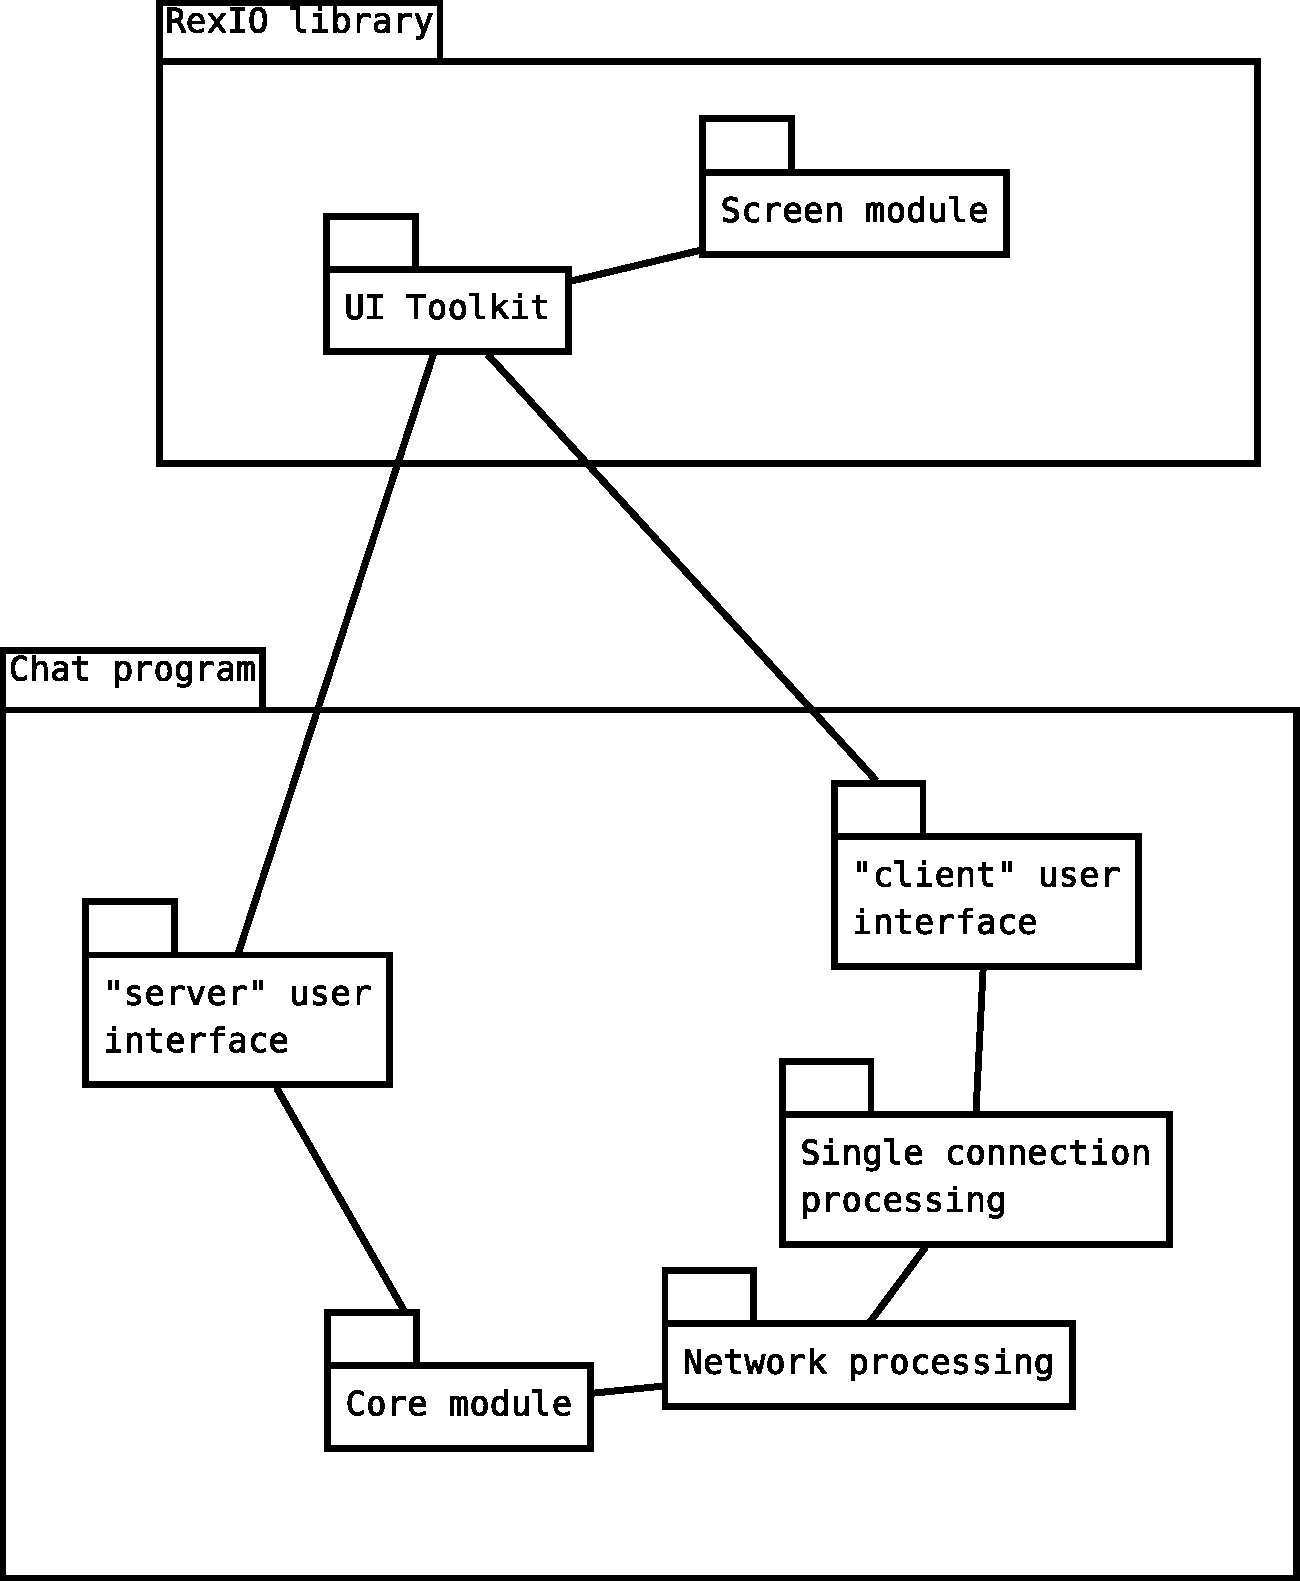
\includegraphics[width=280pt]{graphics/ChatProgram}
  \end{center}
\end{figure}

To run program type for example:
\begin{verbatim}
./test/5/bin/test  -style=test/5/style.rxs -port=4555
\end{verbatim}
  
\verb -style option specifies resource file to be used while
processing connections. This resource file specifies not only colours
of widgets, but also textual values, so it may be used for
internationalization. 

\fullcode
\subsection{Example program listing}
In RexIO distribution this program is located in test/5 directory
\subsubsection{include/main.h++}
\lstinputlisting{../../test/5/include/main.h++}


\subsubsection{include/manager.h++}
\lstinputlisting{../../test/5/include/manager.h++}

\subsubsection{include/demo.h++}
\lstinputlisting{../../test/5/include/demo.h++}


\subsubsection{include/netconn.h++}
\lstinputlisting{../../test/5/include/netconn.h++}


\subsubsection{src/main.c++}
\lstinputlisting{../../test/5/src/main.c++} 


\subsubsection{src/manager.c++}
\lstinputlisting{../../test/5/src/manager.c++}

\subsubsection{src/demo.c++}
\lstinputlisting{../../test/5/src/demo.c++}


\subsubsection{src/netconn.c++}
\lstinputlisting{../../test/5/src/netconn.c++}


\subsubsection{src/netconn.c++}
\lstinputlisting{../../test/5/src/netconn.c++}

\subsubsection{style.rxs}
\begin{verbatim}
RootWindow {
    style: Black Dark Green;
}

FramedWindow {
    style: Red Bright Black;
    frameColor: White Dark Red;
}

LoginWindow {
    style: Red Bright Black;
    frameColor: White Dark Red;
}

Label#welcome {
    style: Yellow Bright Transparent;
    content: "Witaj w aplikacji testowej RexIO";
}

Label#welcome2 {
    style: Yellow Bright Transparent;
    content: "Witaj w aplikacji do pogawędek RexIO!";
}

Inputbox#nickinput {
    style: White Dark Blue;
    cursorStyle: Yellow Bright Yellow;
    activeStyle: White Bright Blue;
}

Button#okbutton {
    style: White Dark Blue;
    activeStyle: White Bright Blue;
}

Label#info0 { content: "Demo to ukazaje działanie RexIO na przykładzie";}
Label#info1 { content: "sieciowej aplikacji do pogawędek.";}
Label#info2 { content: "Interfejs graficzny udostępniany jest przez";}
Label#info3 { content: "zwykły klient "telnet".";}
Label#info5 { style: Magenta Bright Transparent; }
Label#info6 { content: "Użyj telnet by połączyć się z powyższym portem.";}

Label#info15 { content: "Miłego użytkowania!"; }

Label#rexio1 { content: "RexIO jest biblioteką kontroli interfejsu";}
Label#rexio2 { content: "tekstowego z wsparciem dla szerokiej gamy";}
Label#rexio3 { content: "terminali oraz sposobów łączenia. Terminale";}
Label#rexio4 { content: "zdalne jak i lokalne obsługiwane są przez";}
Label#rexio5 { content: "klasy o takim samym interfejsie.";}

RexLogo { style: Cyan Bright Transparent; }

Label#infobar {
    style: White Bright Yellow;
}

Inputbox#msginput {
    style: White Dark Blue;
    cursorStyle: Yellow Bright Yellow;
    activeStyle: White Bright Blue;
}

NickList {
    style: Yellow Bright Red;
    nickColor: Magenta Bright Transparent;
}
\end{verbatim}



\pagebreak
\subsection{Screenshots}
  \index{screenshot}
Server welcome screen
  \begin{figure}[H]
  \begin{center}
  \leavevmode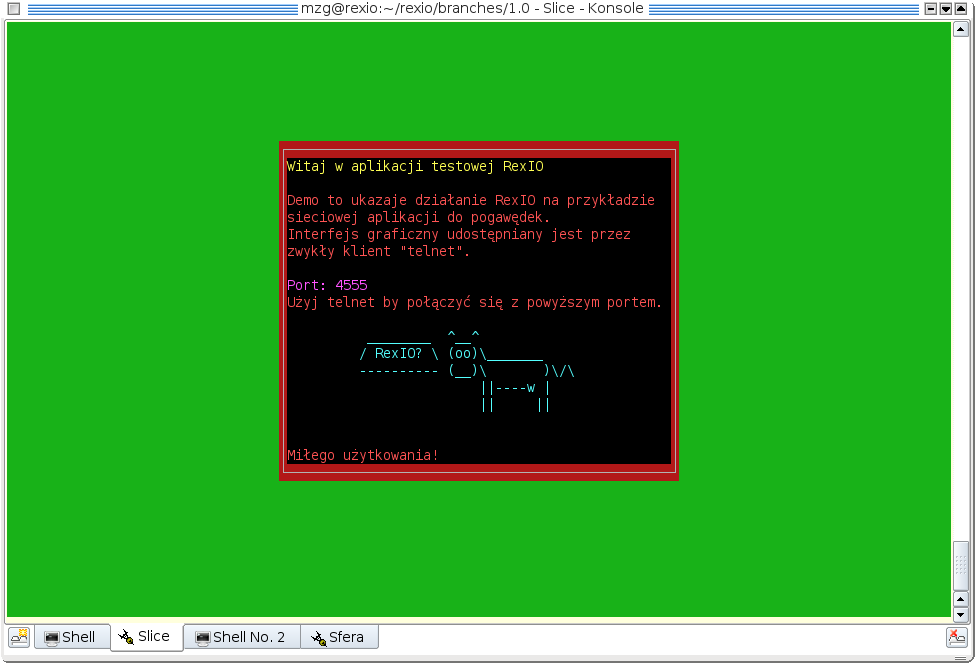
\includegraphics[width=320pt]{graphics/ChatServer}
  \end{center}
  \end{figure}


Client welcome screen
  \begin{figure}[H]
  \begin{center}
  \leavevmode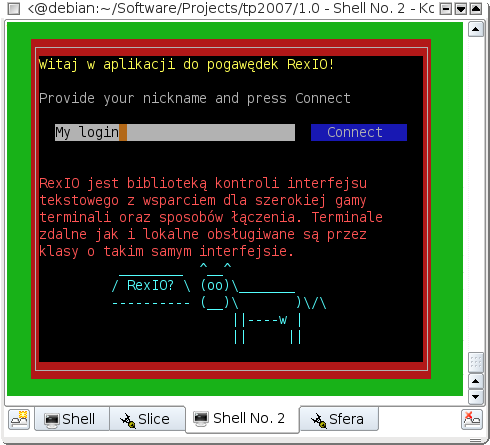
\includegraphics[width=270pt]{graphics/ChatLogin}
  \end{center}
  \end{figure}

\pagebreak
  \index{screenshot}
Client default chat screen
  \begin{figure}[H]
  \begin{center}
  \leavevmode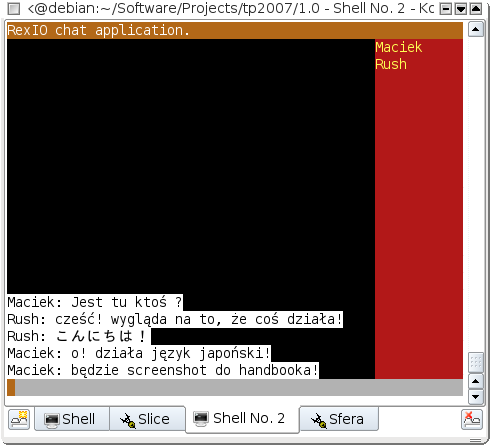
\includegraphics[width=270pt]{graphics/Chat}
  \end{center}
  \end{figure}

\cleardoublepage



\section{References}
Following works are included in the library:
\begin{itemize}
\item \_\_WHERE\_AM\_I\_\_ macro was originally written by  Curtis Krauskopf
\item fileno\_hack function was originally written by Richard B. Kreckel
\item Scr::TI::Strings, Scr::TI::Numbers and Scr::TI::Booleans enums
  are  based on macros in  /usr/include/term.h file, by Zeyd M. Ben-Halim, Eric
 S. Raymond and Thomas E. Dickey.
\item Scr::LocalScreen::TestForResize member function is based on
  comparable function in Berkley TELNET client.
\end{itemize}
\index{references}
\index{bibliography|see{references}}
\cleardoublepage

\printindex

\end{document}














